\chapter{ページング}
% セグメンテーションはプロセスに複数のアドレス空間を持たせ,
% それぞれに役割りに応じた性質を持たせたり,
% 独立して大きさを変化させることで,
% 使いやすいメモリを提供した.
% しかし,物理メモリより大きなセグメントを作ることができない,
% 外部フラグメンテーションが発生する等の問題もあった.
% 
メモリを一様なページに分割し,
ページ単位で管理することで使いやすい仮想メモリを提供する.
メモリより大きな仮想アドレス空間を使用でき,
%外部フラグメンテーションを生じない,
メモリコンパクションが不要なメモリ管理方式である.
Windows,macOS,Linux等の多くのオペレーティングシステムが
ページングを採用している.

%==========================================================================
\section{基本概念}
\figref{pageToFrame}に示すように,
プロセスの仮想アドレス空間は固定サイズの\emph{ページ}に分割される.
物理アドレス空間もページと同じサイズの\emph{フレーム}\footnote{
「フレーム」は,「物理ページ」,「ページフレーム」と呼ばれることもある.
}に分割される.
ページはフレームにマッピングされる.

\myfigure{btp}{scale=0.66}{Fig/pageToFrame-crop.pdf}
{ページからフレームへのマッピング}{pageToFrame}

\subsection{ページとフレーム}
通常,ページのサイズは2の累乗にする.
これにより,仮想アドレスの上位ビットをページ番号,
下位ビットをページ内アドレスに分割して扱うことができる.
物理アドレスでは上位ビットをフレーム番号,
下位ビットをフレーム内アドレスに分割して扱う.
\figref{pagingAddress}に,
32ビットの仮想アドレスを4KiB\footnote{
IA-32のページサイズは基本的に4KiBである.
x86-64でも基本は4KiBである.}のページに分割した例と,
32ビットの物理アドレス空間を4KiBのフレームに分割した例を示す.
4KiBのページ(フレーム)をバイト毎にアドレス付けするためには,
次の計算から分かるように12ビットのページ内(フレーム内)アドレスが必要である.
\centerline{$4KiB = 4 \times 1KiB = 2^2 \times 2^{10}B = 2^{12}B$}
上位20ビットがページ(フレーム)番号を
下位12ビットがページ内(フレーム内)アドレスを表現する.

仮想アドレスのページ番号(p)を
物理アドレスのフレーム番号(f)に変換することで,
ページがフレームにマッピングされる.
\figref{pagingAddress}の例では
仮想アドレスも物理アドレスも同じ32ビットであるが,
異なるサイズでも構わない\footnote{
同じアーキテクチャですら,時期によって関係が変化することがある.
IA-32の物理アドレスは,当初は32ビットであったが途中から36ビットに変更された.
この間,論理アドレスは32ビットのまま変更されていない.}.
\figref{pageToFrame}は物理アドレス空間の方が広い例になっていた.

\myfigure{btp}{scale=0.66}{Fig/pagingAddress-crop.pdf}
{ページング使用時のアドレス例}{pagingAddress}

\subsection{マッピング関数}
仮想アドレス由来のページ番号(p)を,
物理アドレスの一部であるフレーム番号(f)にマッピングする.
マッピング関数はページテーブルと呼ばれる表として実装する.
メモリ管理ハードウェア(MMU:Memory Managiment Unit)が
実行時にページテーブルを参照し動的にマッピングを行う.

プロセス毎に異なる仮想アドレス空間をマッピングするので,
プロセス毎に異なるマッピング関数(ページテーブル)が必要である.
ディスパッチャはプロセスの実行を開始する前にMMUを操作し,
新しいプロセスのマッピング関数を有効にする必要がある.
\figref{pageToFrame}の例では,
プロセスA実行時にはページ0がフレーム1へマッピングされる関数を使用するが,
プロセスB実行時にはページ0がフレーム4へマッピングされる関数に切り換える
必要がある.

\subsection{外部フラグメンテーション}
全てのフレームは,
任意のプロセスの任意のページにマッピング可能である.
連続したフレームが存在しないと使用できない等の制約は無いので
フレームが無駄になることはない.
ページングを用いることで
割り付け単位(フレーム)の外にフラグメントが発生しなくなる.
\emph{外部フラグメンテーション問題は解決し
メモリコンパクションも不要になった}.

\subsection{内部フラグメンテーション}
例えばUNIXプロセスの仮想アドレス空間は,
\figref{pagingInnerFragment}のように配置される.
プログラム領域はページ0からページ1の途中までを使用する.
これらのページは読み出しと実行だけ(r-x)ができるようにメモリ保護を行う.
データとヒープは読み出しと書き込みだけ(rw-)ができるようにするので,
プログラムとは異なるページに配置する必要がある.
そこで,ページ1の後半は使用しないで,ページ2からページ4にデータを配置する.
ページ5からページn-1までは使用しないのでフレームを割り付けない.
仮想アドレス空間に穴が空いた状態にする\footnote{
\emph{sparse address spaces}と呼ばれる.}.
スタックはページnに割り付ける.

以上のように配置すると,
ページ1の後半,ページ4の後半,ページnの前半に,
フレームが割り付けられているにも係わらず使用されない領域ができる.
このようにページ内部(フレーム内部)に無駄な領域が発生することを
\emph{内部フラグメンテーション}と呼ぶ.
フラグメント領域は使用されないはずだが,
ユーザプログラムが誤ってアクセスするかもしれない.
ページングではメモリ保護をページ単位で行うので,
このような不正なアクセスを検知できない問題がある.

\myfigure{btp}{scale=0.66}{Fig/pagingInnerFragment-crop.pdf}
{ページング使用時の仮想アドレス空間の例}{pagingInnerFragment}

%==========================================================================
\section{ページング機構}
以上で説明したページングを実現するためのハードウェア機構について考える.

\subsection{ページング機構の概要}
\figref{paging}にページング機構の模式図を示す.
CPUが出力した仮想アドレスは,
パージ番号(p)とページ内アドレス(w)に分けられる.
ページ番号は,
ページテーブルから一つのエントリを選択するためのインデクスとして使用される.
選択されたエントリのフレーム番号(f)フィールドと
ページ内アドレス(w)を結合して物理アドレスを得る.

\myfigure{btp}{scale=0.66}{Fig/paging-crop.pdf}
{ページング機構の概要}{paging}

\subsection{ページテーブルエントリ}
ページテーブルのエントリはページ番号で選択する.
エントリの内容はc(制御)とf(フレーム番号)フィールドである.
fフィールドの内容がページテーブルの出力になる.

cフィールドの内容は,例えば\tabref{pageTableAttr}のようなものである.
ページにフレームが割り付けられていない場合はVビットが0になっている.
Vビットが0のページにアクセスした場合はCPUに\emph{ページ不在割込み}を発生する.
Rビットはページが参照された時に1に変化する.
Rビットはページの使用頻度を調べるために使用される\footnote{
詳しくは仮想記憶の章で説明する.}.
Dビットはページが書き換えられた時に1に変化する.
Dビットはページをスワップアウトする際に使用される.

\begin{mytable}{btp}{ページテーブルのCフィールドの例}{pageTableAttr}
  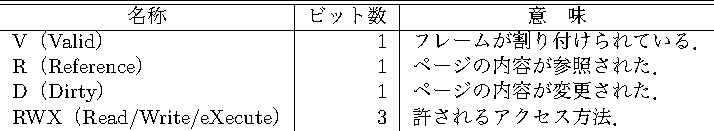
\includegraphics[scale=1.0]{Tbl/pageTableAttr.pdf}
\end{mytable}

\subsection{ページテーブル}
ページテーブルはかなり大きな表である.
例えば\figref{pagingAddress}のようにページ番号が20ビットで表現されるなら,
ページテーブルは$2^{20}=2Mi$エントリの大きさを持つことになる.
また,メモリアクセスの度に参照されるので,
通常のメモリと比較して桁違いに高速でなければならない.

\figref{paging}ではページテーブルが専用のハードウァのように描かれているが,
このような大きくて高速な表をMMUの内部に持つことは困難である.
また,プロセス毎にページテーブルが必要なので,
プロセススイッチの度にページテーブル全体をMMUにロードし直すのも効率が悪い.
そこで,ページテーブルはメモリ上に置くことになる.
ページテーブルのアドレスは\emph{ページテーブルレジスタ}が記憶している.

\subsection{TLB(Translation Look-aside Buffer)}
CPUがメモリをアクセスする度にメモリ上のページテーブルをアクセスすると,
メモリのアクセス回数が二倍になる\footnote{
セグメントテーブルの章で説明したことと同じである.}.
そこで,
変換結果をMMU内の\emph{TLB}と呼ばれる高速なメモリにキャッシュするようにする.
TLBはページ番号とフレーム番号の対応表を記憶し,
ページ番号をキーにして非常に高速に検索できる特殊なメモリである.
このような記憶したキーで高速に検索できるメモリを\emph{連想メモリ}と呼ぶ.
TLBのサイズは機種により異なり,
数十エントリから数千エントリ程度である.

\figref{pagingWithTlb}にTLBを使用したページング機構の模式図を示す.
CPUが出力したページ番号を用いてTLBを検索し,
見つかればTLBからフレーム番号が出力される.
その際,TLB上にコピーされたD(Dirty)ビットが操作されたり,
R/W/Xフィールドがチェックされたりする.
チェックの結果,違反が見つかればCPUに割込みを発生する.

\myfigure{btp}{scale=0.66}{Fig/pagingWithTlb-crop.pdf}
{TLBを使用するページング機構}{pagingWithTlb}

\subsection{Page Table Walk}
ページ番号がTLBに見つからない場合は,
\emph{TLB miss}になりページテーブル上を検索する必要がある.
ページテーブル上の検索のことを\emph{page table walk}と呼ぶ.
page table walk を行いTLBを更新する作業を
MMUのハードウェアが自動的に行う機種と,
CPUに割込みを発生しソフトウェアで行う機種がある.
前者はハードウェアで行うことで高速化を狙う.
後者はMMUを単純にしたことで余ったチップ面積を
TLBのエントリ数を増やすために使用し
TLB miss の頻度を低くすることを狙う.

TLBに空きエントリが無い場合,
新しいページテーブルエントリをロードする前に,
どれかのエントリをTLBから捨てる必要がある.
TLB上のページテーブルエントリのコピーは,
ロードされた後にD(Dirty)ビットが変更されている可能性がある.
TLBのエントリをメモリ上のページテーブルに書き戻すことがある.

\subsection{TLBエントリのクリア}
プロセスは専用の仮想アドレス空間を持つので,
プロセス毎に専用のページテーブルを持つことになる.
プロセススイッチ時に,
ディスパッチャが新しいプロセスのページテーブルのアドレスを
ページテーブルレジスタにロードする.

TLBは古いページテーブルの内容を反映しているので,
ページテーブルを交換する前にクリアする.
TLBの全てのエントリがクリアされると,
直後に同じプロセスに戻ってきた場合や,
カーネル領域などがプロセス間で共有される場合に効率が悪いので
様々な工夫\footnote{
TLBのエントリにプロセス番号も記録しクリア不要にする方式や,
仮想アドレスを指定して特定のエントリだけクリアする方式が知られている.
}が凝らされている場合もあるが,
基本的にはプロセススイッチを行う際はTLBをクリアする.
また,ページテーブルが変更された場合は,
プロセススイッチが発生しなくてもTLBをクリアする必要がある.

\section{ページの共用}
セグメンテーションではプロセスがセグメントを共用することができた.
ページングではプロセス間でページを共用することができる.
\figref{pageSharing}は,
プロセスAとプロセスBが同じプログラムXを,
プロセスCがプログラムC実行している例である.
各プロセスのページテーブルを適切に設定することで,
図のようなマッピングをすることができる.

\myfigure{btp}{scale=0.66}{Fig/pageSharing-crop.pdf}
{プロセス間でのページ共用}{pageSharing}

プログラム本体やライブラリの機械語は読み出しと実行専用(R-X)になっており,
プロセスが変更することは無いので共用することができる.
プログラムXの機械語は第1フレームに格納されプロセスAとプロセスBで共用する.
プログラムCの機械語は第4フレームと第7フレームを合わせた領域に格納される.
プログラムCを実行するプロセスは他に無いので共用する必要がない.

ライブラリの機械語は第3フレームに格納されプロセスA,プロセスB,
プロセスCが共用して利用する.
ライブラリはプロセスA・BとプロセスCで異なる仮想アドレスにマッピングされている.
ライブラリ内の機械語プログラムは何番地にロードされても実行できる
\emph{位置独立コード}\footnote{
JMPやCALL命令のアドレッシングは全てプログラムカウンタ相対で行う.
データのアドレッシングはCPUレジスタに格納したアドレスを基準にした相対で行う.
}でなければならない.
セグメンテーションには,このような制約は無かった.

プロセス毎に内容が異なるデータやスタックは共用できない.
プロセス毎に専用の領域を割当てる.

%==========================================================================
\section{ページテーブルの編成方法}
\figref{pagingWithTlb}に示したようにページテーブルはメモリに置かれる.
しかし,ページテーブルのサイズは無視できるほど小さなものではない.
例えば,32ビットマイクロプロセッサがPCに普及してきた1990年代の前半には,
PCが備えるメモリは4MiBから16MiB程度であった.
IA-32を用いる場合,ページテーブルの一つのエントリは4バイトなので,
32ビットの仮想アドレス空間を4KiBのページで分割すると,
次の計算のようにページテーブル全体では4MiBになる.
更に,ページテーブルはプロセス毎に必要である.
メモリのほとんどをページテーブルに使用しても足らない.
このままでは実用にならない.

\centerline{$2^{32}B \div 2^{12}B = 2^{20} = 1Miエントリ$}
\centerline{$1Miエントリ \times 4B = 4MiB$}

近年の64ビットマイクロプロセッサの場合も同様である.
x86-64では48ビットの仮想アドレス空間を4KiBのページで分割する.
ページテーブルの一つのエントリが8バイトなので,
下の計算のようにページテーブルのサイズが512GiBになる.
これでは現代のPCにもページテーブルが大きすぎる.
ページテーブルを小さくする必要がある.

\centerline{$2^{48}B \div 2^{12}B = 2^{36} = 64Giエントリ$}
\centerline{$64Giエントリ \times 8B = 512GiB$}

\subsection{二段のページテーブル}
ページテーブルを二段にすることで,
二段目に使用するメモリを節約することができる.
\figref{pagingMultiLevel}にIA-32で使用される二段のページテーブルの例を示す
\footnote{\figref{pagingMultiLevel}ではIA-32の用語ではなく,
より一般的な用語を使用している.}.
図の左上に示すように,
32ビットの仮想アドレスは10ビットのページ番号フィールド二つ(p,q)と,
12ビットのページ内アドレス(w)に分けられる.
ページサイズはwが12ビットなので$2^{12}=4KiB$である.
物理アドレスも32ビット\footnote{
初期のIA-32の場合である.途中から36ビットに拡張された.
}なので,フレーム番号は20ビットで表現する.

\myfigure{btp}{scale=0.5}{Fig/pagingMultiLevel-crop.pdf}
{二段ページテーブルの構造}{pagingMultiLevel}

\begin{itemize}
\item \emph{Page Table Walk} \\
まず,ページテーブルレジスタから一段目のページテーブルの位置を知る.
次に,一段目のページテーブルをpをインデクスにして参照することで,
二段目のページテーブルの位置を知ることができる.
最後に,二段目のページテーブルをqをインデクスにして参照することで,
フレームの位置を知る.
フレームのwバイト目が目的のアドレスである.
このように二つのページテーブルを用いた page table walk を行うことで
目的の物理アドレスに辿り着く.

\item \emph{一段目のページテーブル} \\
一段目のページテーブルの大きさは,pが10ビット,
エントリサイズが4バイトより$2^{10} \times 4B =4KiB$になる.
これは,ちょうどフレームと同じ大きさであり実際に1フレームに格納する.
よって,ページテーブルレジスタは
一段目ページテーブルのフレーム番号(10ビット)を記録する.

\item \emph{二段目のページテーブル} \\
一段目のページテーブルの一つのエントリが,
二段目のページテーブルの一つの区画を選択する.
区画は10ビットのqを用いて参照されるので,
大きさは一段目のページテーブルと同じ$4KiB$になる.
区画も一つのフレームに格納される.
一段目のページテーブルのfフィールドには,
二段目ページテーブルの一つの区画のフレーム番号(10ビット)を格納する.

\item \emph{メモリの節約}\\
\figref{pagingInnerFragment}や\figref{pageSharing}で示したように,
プロセスの仮想アドレス空間には
フレームが割り付けられていない大きな穴が空いている.
\figref{pagingSparseSpace}のように,
穴の部分に二段目のページテーブルを割当てないことでメモリを節約できる.
図の例では一段目と二段目合わせて3フレームしか
ページテーブルのために使用していない.
もしも,二段目のページを全て割り付けたなら
$2^{10}+1=1,025$フレームを使用するので効果は大きい.
また,二段目のページテーブルとフレームで使用頻度の低いものを
二次記憶装置にスワップアウトすることも可能である\footnote{
詳しくは仮想記憶の章で述べる.}.

\myfigure{btp}{scale=0.66}{Fig/pagingSparseSpace-crop.pdf}
{穴空き仮想アドレス空間のページテーブル}{pagingSparseSpace}
\end{itemize}

\subsection{多段ページテーブル}
前の節では二段のページテーブルを紹介した.
仮想アドレス空間が更に広い場合は,
より段数の多いページテーブルが使用されることがある.
例えば,
x86-64では64ビット(実質的には48ビット)\footnote{
\figref{paging4Level}に示すように
64ビットの上位16ビットは未使用なので,
実質的な仮想アドレスは48ビットになる.
$2^{48}B = 2^8 \times 2^{40}B = 256TiB$なので,
48ビットでも十分に広いアドレス空間である.
}の広い仮想アドレス空間が使用できる.
IA-32では仮想アドレス空間が32ビットだったので
4GiBより大きなプロセス(セグメント)を作ることはできなかった.
x86-64ではより大きなプロセスを作ることができるので,
4GiBの上限を気にしないでプログラミングできる.

しかし,二段のページテーブルを使用し続けると,
ページテーブルの区画が大きくなりメモリの無駄が多くなる.
例えば,仮想アドレスが48ビット,二段のページテーブルを用い,
エントリのサイズが8バイトと仮定する.
48ビットの仮想アドレスを,
18ビット(p),18ビット(q),12ビット(w)に分割して扱う場合,
ページテーブル一区画のサイズは$2^{18} \times 8B = 2MiB$となる.
\figref{pagingSparseSpace}と同様な考えで,
最低限である3区画がページテーブルに割当てられたとすると
プロセス当たり12MiBになる.
システム内にプロセスが400個\footnote{
この原稿を書いているMacBookでは,現在354個のプロセスが走っている.
}あったとすると,
最低でも4.8GiBのメモリがページテーブルのために消費されることになる.
ページテーブルに使用されるメモリが多すぎる\footnote{
この原稿を書いているMacBookのメモリは8GiBであるので,
仮定どおりなら半分以上がページテーブルに消費されることになる.
}.

ページテーブルの区画を小さくするために仮想アドレスをより小さく区切る.
例えば,x86-64では\figref{paging4Level}のよう
仮想アドレスのページ番号部分を四つに区切っている.
ページ内アドレスが12ビットなので,
ここでもページ(フレーム)サイズは4KiBである.
ページテーブルは9ビットの
p1,p2,p3,p4でインデクスされるので512エントリである.
エントリサイズはx86-64の場合8バイトなので,
ページテーブルは4KiBになりフレームサイズと同じになる.
\figref{pagingSparseSpace}と同様な仮想アドレス空間をマッピングする場合,
ページテーブルに使用するメモリは,
1段目に1フレーム,
2段目に2フレーム,
3段目に2フレーム,
4段目に2フレームの合計7フレーム(28KiB)で済む.
プロセスが400個あったとしても,
ページテーブルに使用するメモリの合計は約11MiBにしかならない.

\myfigure{btp}{scale=0.5}{Fig/paging4Level-crop.pdf}
{四段のページテーブルの例}{paging4Level}

\subsection{逆引きページテーブル}
従来のページテーブルは,
仮想アドレス空間の大きさにより大きくなるし,
仮想アドレス空間の数だけ必要である.
これは,仮想アドレスから物理アドレスに変換するために,
仮想アドレス(ページ番号)をインデクスとし
物理アドレス(フレーム番号)を内容とする表を,
仮想アドレス空間毎に用いる自然な発想から生まれた.

逆引きページテーブルは,
従来のページテーブルとは逆に,
物理アドレス(フレーム番号)をインデクスとし,
仮想アドレス(ページ番号)を内容とする表を
システム全体で一つだけ用いる方式である.
ページテーブルのエントリ数はフレーム数と等しくなるので,
ページテーブルが使用する領域の大きさは小さく,かつ,一定である.

\cite{invertedPageTable}

%==========================================================================
%\newpage
\section*{問題}
スタックセグメントを意識した
\emph{前向きに伸びるセグメント}も利用可能な
セグメンテーション機構を設計しなさい.

\begin{enumerate}
\item セグメントテーブルに必要な変更は?
\item \figref{segmentation}に必要な変更は?
\item 他に必要な変更は?
\end{enumerate}
